\chapter{Testes e Resultados}
\label{ch::test-result}

\section{Introdução}
\label{sec::test-result:intro}

A implementação das funções e dos \textit{scripts} do projeto e respetiva execução com os hologramas selecionados para este culmina no cumprimento do \ref{obj:avaliar_psnr}\textordmasculine~e último objetivo secundário do projeto, o qual permitirá retirar conclusões para o objetivo primário identificado na Secção \ref{sec::intro:objs}.

Para tal, ir-se-ão resumir os testes efetuados (Secção \ref{sec::test-result:test}) e os resultados de si obtidos (Secção \ref{sec::test-result:result}), assim como discuti-los na perspetiva do objetivo do projeto (Secção \ref{sec::test-result:discussao}).


\section{Testes}
\label{sec::test-result:test}

A sequência de fases de investigação apresentada no Capítulo \ref{ch::imp-test} e resumida na \textit{pipeline} ilustrada pela Figura \ref{fig:projeto} foi exaustivamente testada com os 3 hologramas enumerados na Secção \ref{ssec::tecno-ferr:materiais:hologramas}.

Os parâmetros apresentados na Tabela \ref{tab:holo-specs} são fixos (a fim de garantir a reconstrução do holograma), sendo a distância de reconstrução (parâmetro \verb|z|) em particular um intervalo. Qualquer valor dentro deste intervalo pode ser tomado. A par deste parâmetro, também o tamanho da vista (valor arbitrário menor do que a resolução do holograma) é necessário para a fase de testes, conforme as funções transcritas e implementadas ao longo do Capítulo \ref{ch::imp-test}. Os valores selecionados para estes dois parâmetros são apresentados na Tabela \ref{tab:teste-parametros}.

\begin{table}[!htbp]
    \centering
    \caption{Parâmetros variáveis utilizados na reconstrução dos hologramas.}
    \label{tab:teste-parametros}
    \begin{tabular}{r c c}
        \toprule
        Holograma & \verb|z| & \verb|pupil_size| \\
        \midrule
        \texttt{Dices4k} & \SI{0.0020}{} & 2048$\times$2048 \\
        %\hline
        \texttt{DiffuseCar4k} & \SI{0.0012}{} & 2048$\times$2048 \\
        %\hline
        \texttt{Piano4k} & \SI{0.0019}{} & 2048$\times$2048 \\
        \bottomrule
    \end{tabular}
    %\bigskip
    \subcaption*{}
    \begin{tabular}{>{\ttfamily}r @{~:~~} l l}
        z & Distância de reconstrução & (em metros) \\
        pupil\_size & Tamanho da vista & (em pixeis) \\
    \end{tabular}
\end{table}

Os ficheiros \ac{JSON} gerados pelos \textit{scripts} previamente implementados armazenam, conforme descrito na Secção \ref{ssec::imp-tes:holo-compress:script}, os resultados doravante explorados na Secção \ref{sec::test-result:result}.


\section{Resultados}
\label{sec::test-result:result}

Os resultados dos testes efetuados são os valores da métrica \ac{PSNR}, em particular um por holograma, por \textit{bitrate} (débito), por vista, e com e sem transformada de cor. No caso deste projeto, tal traduz-se em $3 \times 12 \times 16 \times 2 = 1152$ valores. Ora, esta quantidade de valores é impraticável de ser exposta e devidamente explorada.

Neste sentido, optou-se por se calcular a média dos valores de \ac{PSNR} e o respetivo desvio padrão por cada \textit{bitrate}, o que reduz para $72$ valores, tornando-se alcançável a devida discussão dos resultados do projeto.

Destacam-se as tabelas e figuras que expõem os resultados da investigação. Porquanto as tabelas dispõem os valores das médias da métrica \ac{PSNR} para as 16 vistas reconstruídas por cada \textit{bitrate} e por opção de com ou sem de transformada de cor, as figuras apresentam-nos graficamente. Em particular:

\begin{itemize}
    \item Holograma \texttt{dices4k}: Tabela \ref{tab:res-dices4k} e Figura \ref{fig:res-dices4k};
    \item Holograma \texttt{diffuseCar4k}: Tabela \ref{tab:res-diffusecar4k} e Figura \ref{fig:res-diffusecar4k};
    \item Holograma \texttt{piano4k}: Tabela \ref{tab:res-piano4k} e Figura \ref{fig:res-piano4k}.
\end{itemize}

\begin{table}[!htbp]
    \centering
    \caption{Resultados da métrica \acs{PSNR} para o holograma \texttt{dices4k}.}
    \label{tab:res-dices4k}
    \begin{tabular}{x{2.2cm} x{2.2cm} x{2.2cm} x{2.2cm} x{2.2cm}}
        \toprule
        \multirow{2}{*}{\bfseries\itshape Bitrate} & \multicolumn{2}{c}{\bfseries Sem transformada de cor} & \multicolumn{2}{c}{\bfseries Com transformada de cor} \tabularnewline
        \cmidrule{2-5}
        & \texttt{avg} & \texttt{std} & \texttt{avg} & \texttt{std} \tabularnewline
        \midrule
        0.1 & 25.432 & 3.852   &   24.768 & 3.684 \tabularnewline
        0.3 & 28.513 & 4.772   &   27.071 & 4.662 \tabularnewline
        0.6 & 31.221 & 5.427   &   29.311 & 5.160 \tabularnewline
        1.0 & 33.723 & 5.919   &   31.176 & 5.591 \tabularnewline
        1.5 & 36.210 & 6.160   &   33.000 & 5.870 \tabularnewline
        2.0 & 38.212 & 6.270   &   34.743 & 6.369 \tabularnewline
        2.5 & 39.942 & 6.337   &   35.930 & 6.410 \tabularnewline
        3.0 & 41.418 & 6.116   &   37.445 & 6.658 \tabularnewline
        3.5 & 42.824 & 6.114   &   38.966 & 6.676 \tabularnewline
        4.0 & 44.097 & 5.957   &   39.966 & 6.521 \tabularnewline
        4.5 & 45.310 & 5.704   &   40.962 & 6.645 \tabularnewline
        5.0 & 46.209 & 5.411   &   42.084 & 6.780 \tabularnewline
        \bottomrule
    \end{tabular}
    %\bigskip
    \subcaption*{}
    \begin{tabular}{>{\ttfamily}r @{~:~~} l l}
        avg & Média do \ac{PSNR} & (em \acs{dB}) \\
        std & Desvio padrão & (em \acs{dB}) \\
    \end{tabular}
\end{table}

\begin{figure}[!htbp]
    \centering
    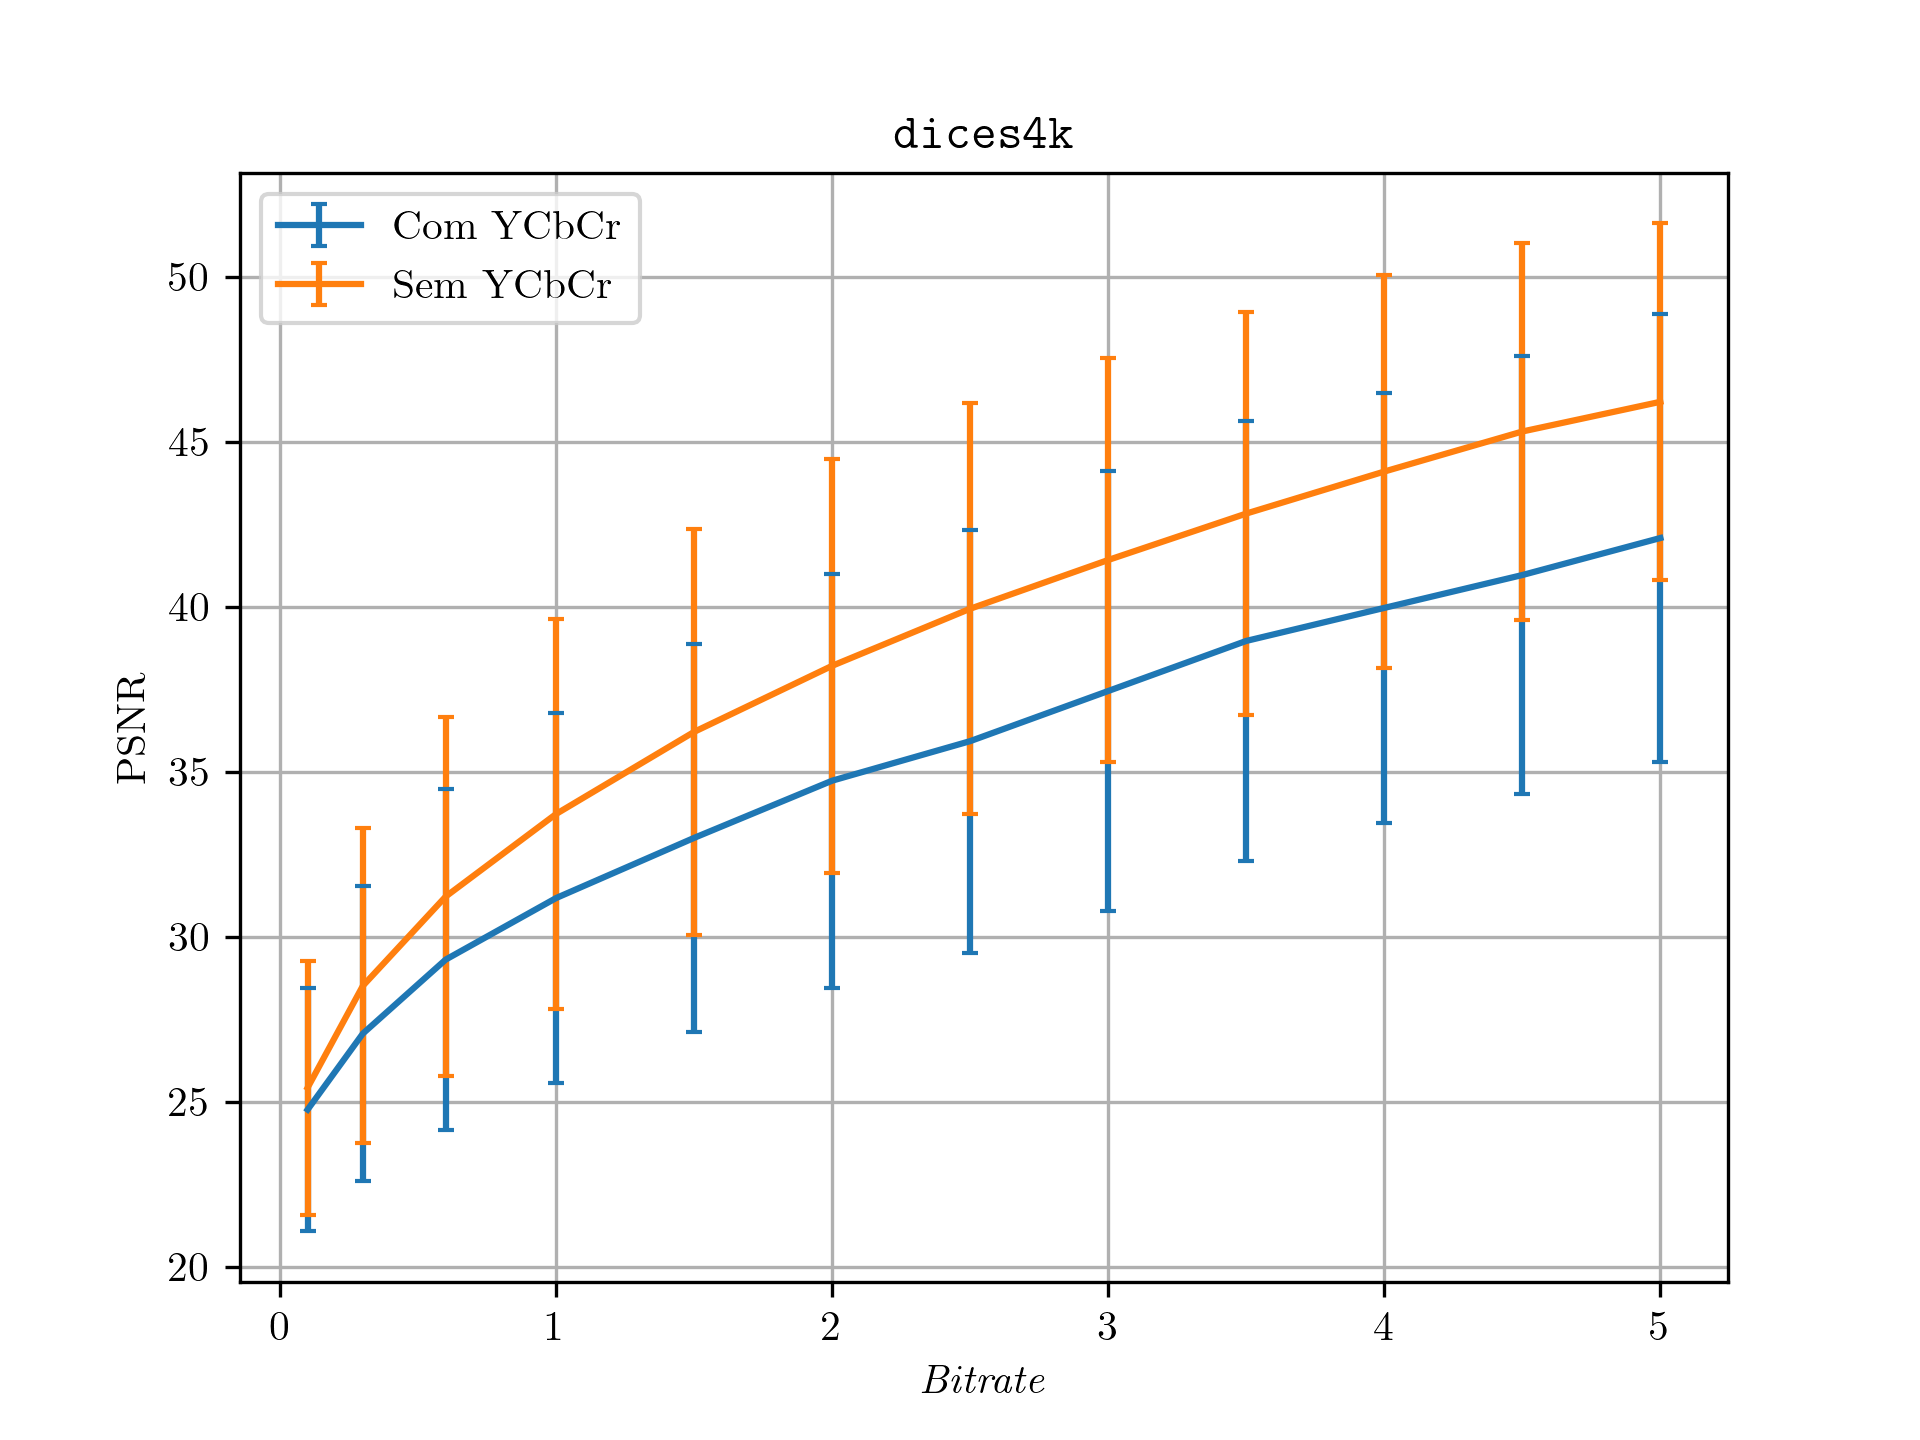
\includegraphics[width=\textwidth]{res_dices4k}
    \caption[Variação da média do \acs{PSNR} relativo ao holograma \texttt{dices4k}.]{Variação da média da métrica \acs{PSNR} relativo ao holograma \texttt{dices4k}. \textit{Valor maior significa melhor qualidade.}}
    \label{fig:res-dices4k}
\end{figure}


\begin{table}[!htbp]
    \centering
    \caption{Resultados da métrica \acs{PSNR} para o holograma \texttt{diffuseCar4k}.}
    \label{tab:res-diffusecar4k}
    \begin{tabular}{x{2.2cm} x{2.2cm} x{2.2cm} x{2.2cm} x{2.2cm}}
        \toprule
        \multirow{2}{*}{\bfseries\itshape Bitrate} & \multicolumn{2}{c}{\bfseries Sem transformada de cor} & \multicolumn{2}{c}{\bfseries Com transformada de cor} \tabularnewline
        \cmidrule{2-5}
        & \texttt{avg} & \texttt{std} & \texttt{avg} & \texttt{std} \tabularnewline
        \midrule
        0.1 & 29.441 & 4.763 & 27.438 & 3.795 \tabularnewline
        0.3 & 33.938 & 6.170 & 29.762 & 5.089 \tabularnewline
        0.6 & 38.299 & 6.820 & 32.336 & 6.019 \tabularnewline
        1.0 & 42.364 & 6.864 & 35.398 & 7.046 \tabularnewline
        1.5 & 46.053 & 6.540 & 38.747 & 7.682 \tabularnewline
        2.0 & 48.611 & 5.938 & 41.496 & 7.635 \tabularnewline
        2.5 & 50.706 & 5.339 & 44.037 & 7.577 \tabularnewline
        3.0 & 52.038 & 4.599 & 45.643 & 6.937 \tabularnewline
        3.5 & 53.174 & 3.899 & 47.263 & 6.262 \tabularnewline
        4.0 & 54.096 & 3.318 & 48.878 & 5.400 \tabularnewline
        4.5 & 54.819 & 2.812 & 50.110 & 4.567 \tabularnewline
        5.0 & 55.280 & 2.310 & 50.851 & 3.706 \tabularnewline
        \bottomrule
    \end{tabular}
    %\bigskip
    \subcaption*{}
    \begin{tabular}{>{\ttfamily}r @{~:~~} l l}
        avg & Média do \ac{PSNR} & (em \acs{dB}) \\
        std & Desvio padrão & (em \acs{dB}) \\
    \end{tabular}
\end{table}

\begin{figure}[!htbp]
    \centering
    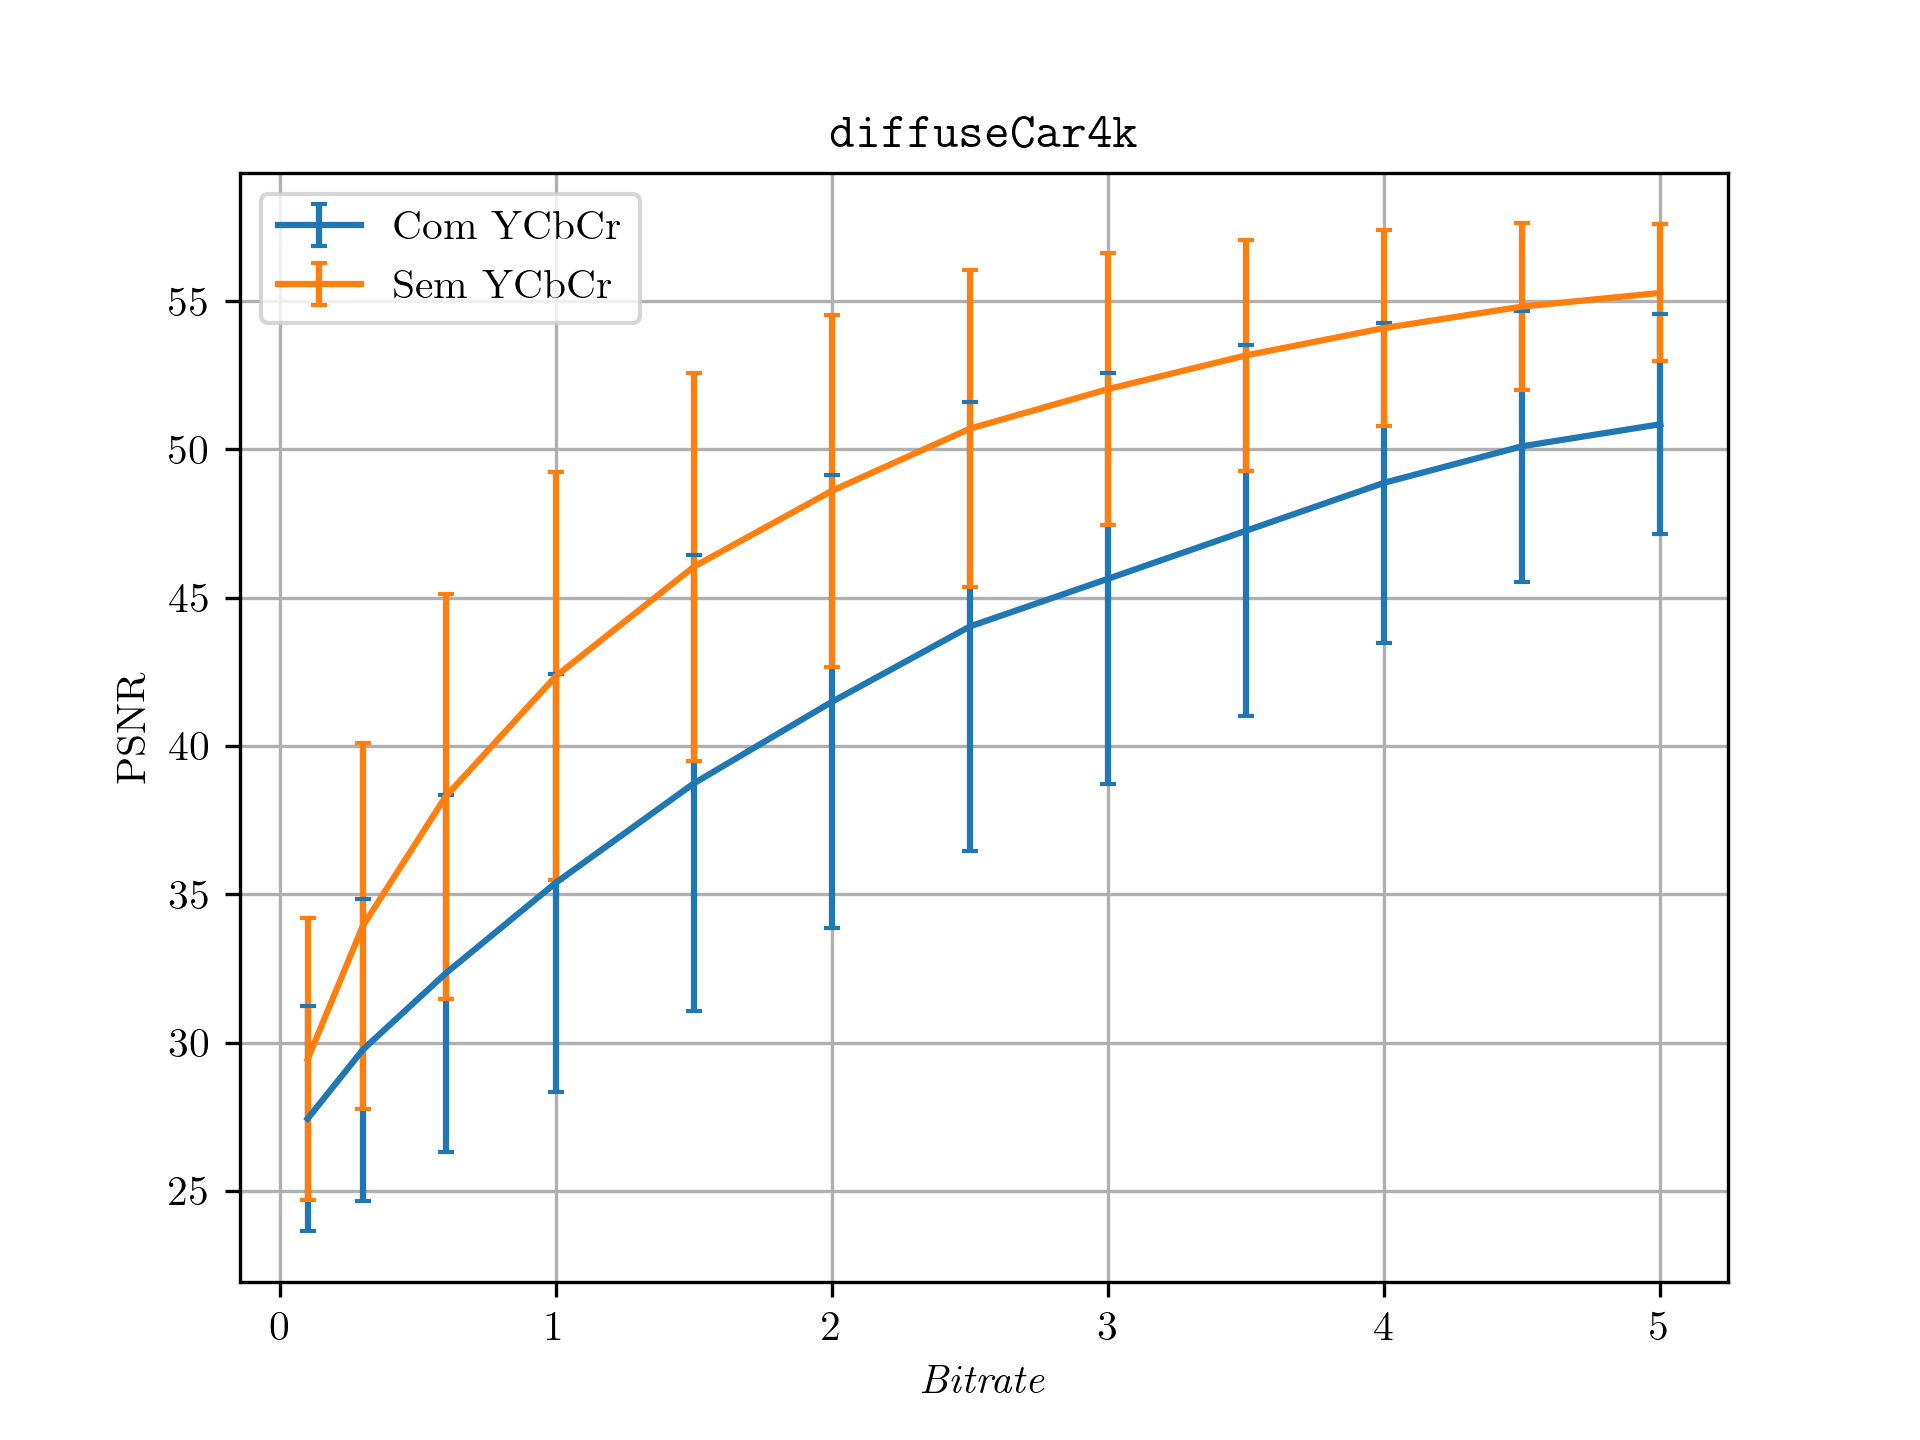
\includegraphics[width=\textwidth]{res_diffuseCar4k}
    \caption[Variação da média do \acs{PSNR} relativo ao holograma \texttt{diffuseCar4k}.]{Variação da média da métrica \acs{PSNR} relativo ao holograma \texttt{diffuseCar4k}. \textit{Valor maior significa melhor qualidade.}}
    \label{fig:res-diffusecar4k}
\end{figure}


\begin{table}[!htbp]
    \centering
    \caption{Resultados da métrica \acs{PSNR} para o holograma \texttt{piano4k}.}
    \label{tab:res-piano4k}
    \begin{tabular}{x{2.2cm} x{2.2cm} x{2.2cm} x{2.2cm} x{2.2cm}}
        \toprule
        \multirow{2}{*}{\bfseries\itshape Bitrate} & \multicolumn{2}{c}{\bfseries Sem transformada de cor} & \multicolumn{2}{c}{\bfseries Com transformada de cor} \tabularnewline
        \cmidrule{2-5}
        & \texttt{avg} & \texttt{std} & \texttt{avg} & \texttt{std} \tabularnewline
        \midrule
        0.1 & 27.352 & 3.958 & 26.156 & 3.579 \tabularnewline
        0.3 & 31.336 & 4.660 & 29.166 & 4.538 \tabularnewline
        0.6 & 34.930 & 4.847 & 31.711 & 4.558 \tabularnewline
        1.0 & 38.291 & 4.827 & 33.782 & 4.631 \tabularnewline
        1.5 & 41.393 & 4.697 & 36.231 & 4.775 \tabularnewline
        2.0 & 43.914 & 4.291 & 38.247 & 4.858 \tabularnewline
        2.5 & 45.947 & 4.019 & 40.340 & 4.911 \tabularnewline
        3.0 & 47.654 & 3.632 & 41.937 & 4.582 \tabularnewline
        3.5 & 48.987 & 3.236 & 43.430 & 4.722 \tabularnewline
        4.0 & 50.300 & 2.873 & 45.279 & 4.550 \tabularnewline
        4.5 & 51.290 & 2.715 & 46.741 & 4.316 \tabularnewline
        5.0 & 52.210 & 2.471 & 47.638 & 3.642 \tabularnewline
        \bottomrule
    \end{tabular}
    %\bigskip
    \subcaption*{}
    \begin{tabular}{>{\ttfamily}r @{~:~~} l l}
        avg & Média do \ac{PSNR} & (em \acs{dB}) \\
        std & Desvio padrão & (em \acs{dB}) \\
    \end{tabular}
\end{table}

\begin{figure}[!htbp]
    \centering
    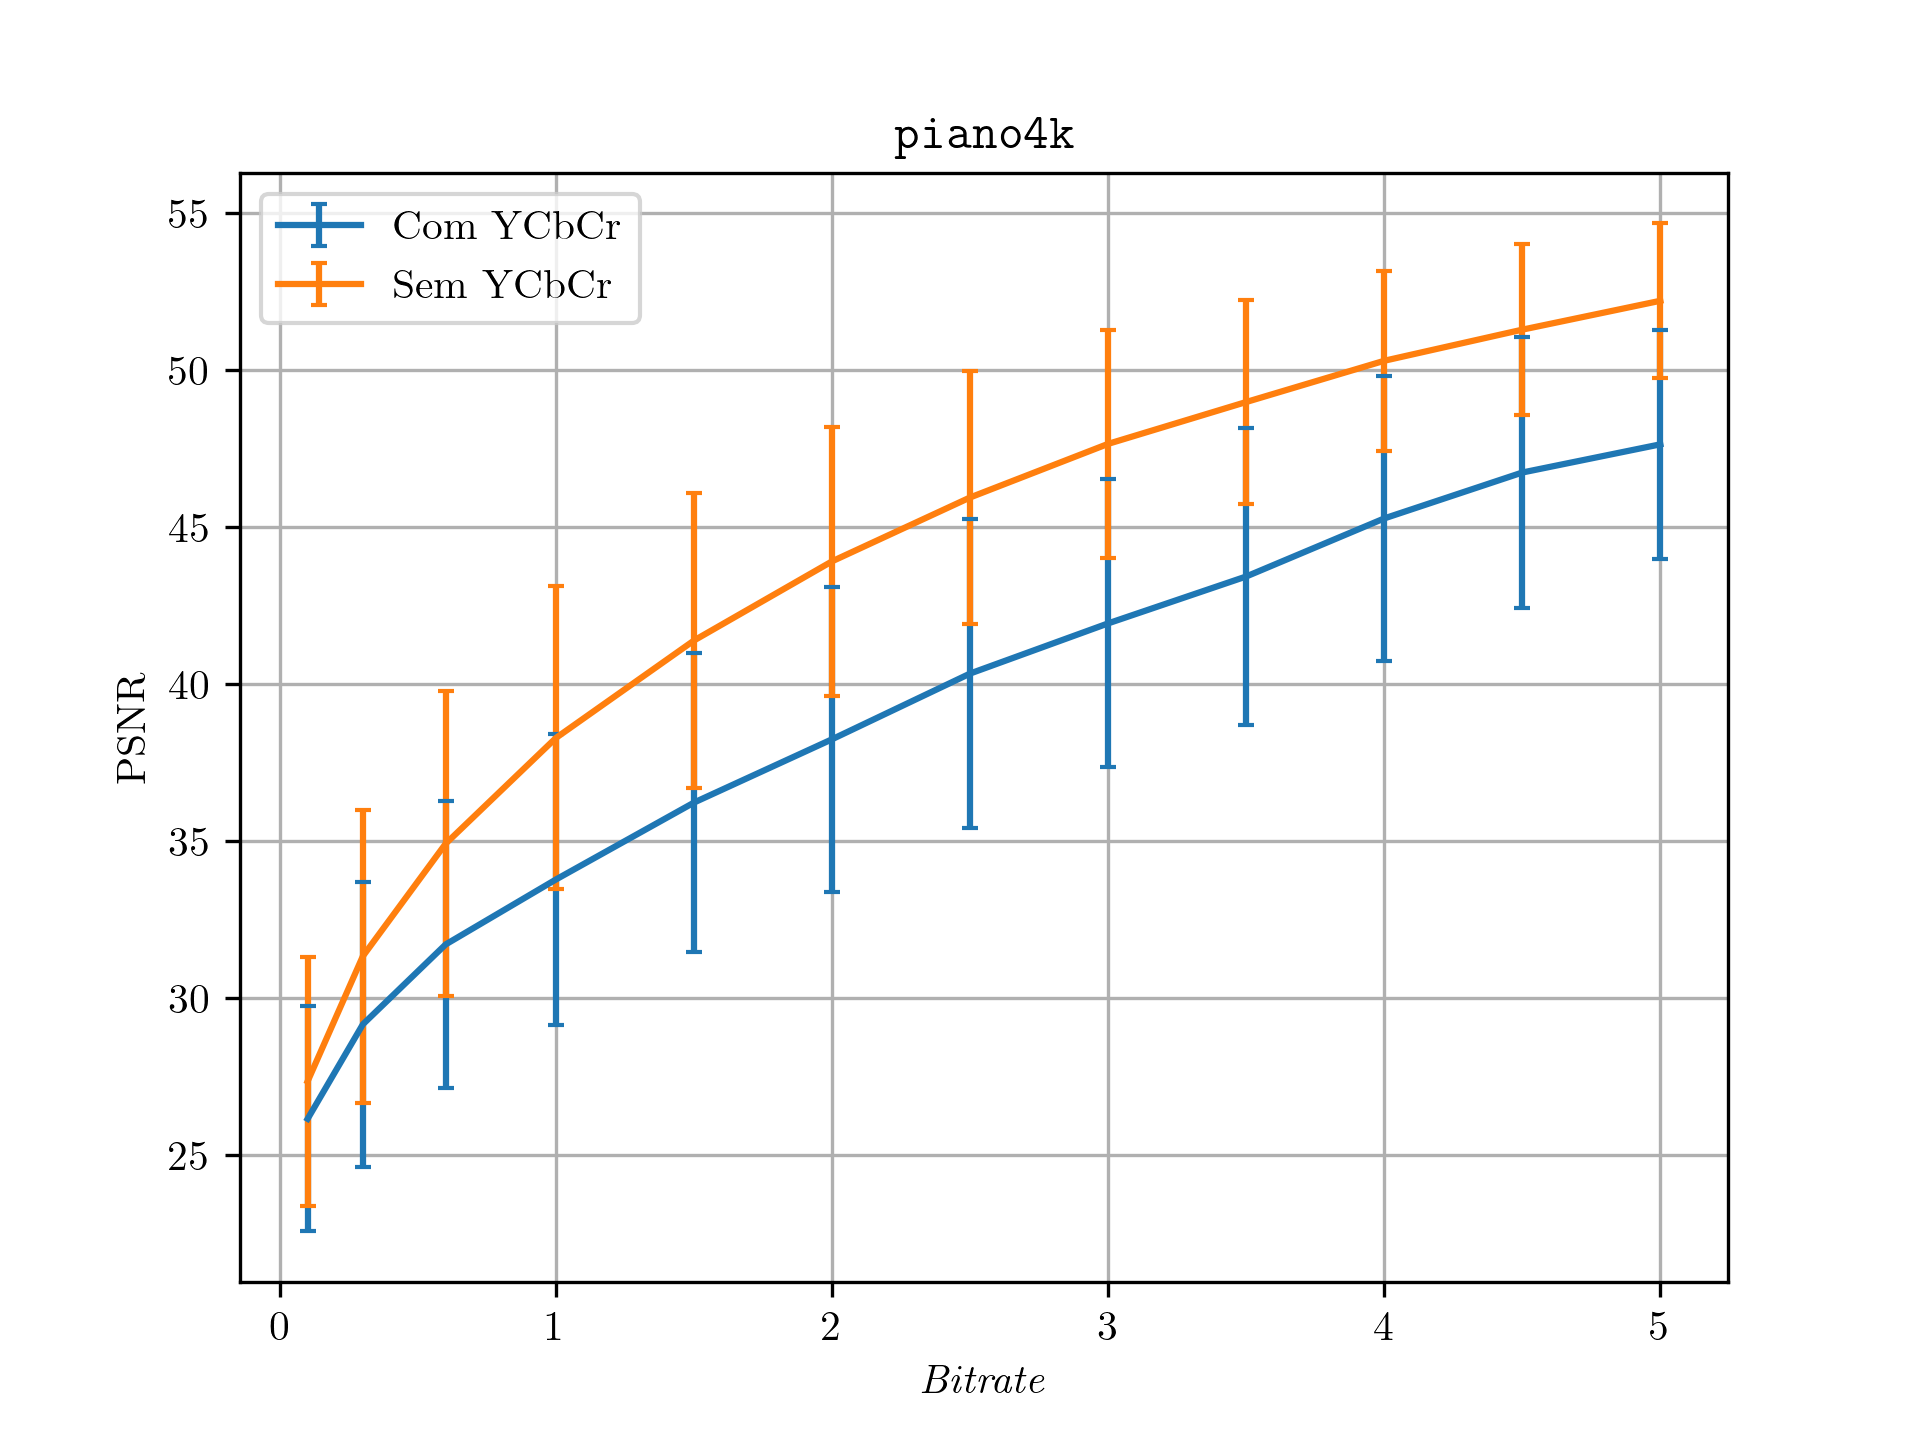
\includegraphics[width=\textwidth]{res_piano4k}
    \caption[Variação da média do \acs{PSNR} relativo ao holograma \texttt{piano4k}.]{Variação da média da métrica \acs{PSNR} relativo ao holograma \texttt{piano4k}. \textit{Valor maior significa melhor qualidade.}}
    \label{fig:res-piano4k}
\end{figure}


\section{Discussão}
\label{sec::test-result:discussao}

Tendo em conta que quanto maior o valor do \ac{PSNR} melhor será a qualidade da imagem após a compressão, uma análise visual aos gráficos das figuras \ref{fig:res-dices4k}, \ref{fig:res-diffusecar4k} e \ref{fig:res-piano4k} permite facilmente observar a diminuição da qualidade de todos os três hologramas testados ao ser utilizada uma transformada de cor de \ac{RGB} para YCbCr.

Há ainda a referir, pela observação das mesmas figuras, que a qualidade dos hologramas comprimidos aumenta com a subida do débito.

%TODO: REVER ESTE PARAGRAFO:\\
%\textbf{
    Tal é conforme o esperado uma vez que o aumento do débito implica a possibilidade de se armazenar uma maior quantidade de informação acerca da imagem original.
%}

Por seu turno, de uma análise mais detalhada às Tabelas \ref{tab:res-dices4k}, \ref{tab:res-diffusecar4k} e \ref{tab:res-piano4k} constata-se a ocorrência de um fenómeno igualmente antecipado nos valores do desvio padrão: este tende a diminuir para \textit{bitrates} mais elevados.



Do exposto, 3 questões colocam-se e que são meritórias de discussão no âmbito da investigação:

\begin{enumerate}
    \item \textit{Qual o motivo para a transformada de cor levar à significativa redução de qualidade após compressão?}\newline
    A transformada de cor de \ac{RGB} para YUV 4:2:0 implica perda de informação nos canais G (\textit{Green}) e B (\textit{Blue}) a fim de tirar partido das características da visão humana. Por si só, esta transformada de cor torna a perda de informação impercetível ao olho humano, sendo esta de uma aparente qualidade equivalente.\newline
    Todavia, a compressão no formato JPEG2000 implica uma nova perda de informação uma vez que este é um formato de compressão com perdas.\newline
    
    
    % COMENTÁRIO
    % Na realidade a transformada de cor de RGB para YUV420 em imagens clássicas não implica grandes perdas a nível do PSNR dada a grande correlação dos pixeis no que diz respeito aos canais U e V, no entanto no caso destes hologramas, em que existe grande quantidade de speckle, mesmo nas vistas, esta correlação diminui e existem perdas neste processo de se acentuam com as etapas seguintes da codificação.

    % ORIGINAL
    % Teoriza-se que a aplicação consecutiva de dois processos que implicam perdas de informação levem a uma significativa redução da qualidade final do holograma comprimido, resultando em valores de \ac{PSNR} claramente inferiores.

    % NOVA VERSÃO (proposta)
    Porquanto a transformada de cor de RGB para YUV 4:2:0 não se traduz numa redução significativa em imagens clássicas, tal não pode ser dito para a holografia. A quantidade de \textit{speckle} (\textit{i.e.} de ruído) nos hologramas leva a que haja uma diminuição da correlação %entre os píxeis originais e os píxeis após a transformada de cor (nomeadamente os canais U e V).
    entre píxeis vizinhos nos canais U e V, levando a que a redução destes coeficientes não seja mais negligenciável no que diz respeito à qualidade final. Tal acaba por se traduzir numa diminuição mais significativa do valor de \ac{PSNR} uma vez que existem perdas que se acentuam nos passos seguintes da compressão.

    É, portanto, teorizado que, no caso dos hologramas, a aplicação consecutiva de dois processos que implicam perdas de informação levem a uma significativa redução da qualidade final do holograma comprimido, resultando em valores de \ac{PSNR} claramente inferiores.

    \item \textit{Por que razão o desvio padrão se revela menor em \emph{bitrates} maiores?}\newline
    O aumento da qualidade dos hologramas comprimidos com \textit{bitrates} maiores (conforme observado anteriormente) dever-se-á explicar pela maior quantidade de informação armazenada. Tal leva à existência de menos ruído nas imagens comprimidas, o que implica uma maior aproximação face à imagem original.\newline
    A par do aumento do \ac{PSNR}, é de denotar que o aumento da informação armazenada deverá implica igualmente uma maior consistência na qualidade dos hologramas comprimidos, independentemente da vista tomada.\newline
    Ora, estatisticamente, uma maior consistência dos dados traduz-se na diminuição do desvio padrão.

    \item \textit{Por que razão o desvio padrão se revela menor em \emph{bitrates} menores?}\newline
    Paralelamente ao ponto anterior, a diminuição do débito introduz um considerável aumento do ruído nos hologramas comprimidos, o que leva a um decaímento rápido do valor de \ac{PSNR} à medida que se diminui o \textit{bitrate} utilizado.\newline
    É, pois, expectável que não existam grandes variações no \ac{PSNR} independentemente da vista tomada na reconstrução do holograma. Por outras palavras, é de esperar consistência na falta de qualidade das imagens (\textit{e.g.} é altamente improvável obter um \ac{PSNR} de \SI{50}{\decibel} quando se obtém consistentemente valores a rondar os \SI{20}{\decibel} para um \textit{bitrate} de \SI{0.1}{}).\newline
    Tal deverá justificar o fenómeno da notória diminuição do desvio padrão para \textit{bitrates} mais baixos.
\end{enumerate}

De referir que a reconstrução em multivista permite verificar que a qualidade de compressão pode igualmente depender da vista a partir da qual é reconstruída.

\section{Conclusões}
\label{sec::test-result:conclusao}

A análise de três grandes variáveis foi levada em consideração durante a investigação e que neste Capítulo foram abordadas:
\begin{enumerate}
    \item Reconstrução em 16 vistas distintas;
    \item Uso de uma transformada de cor de \ac{RGB} para YCbCr;
    \item Uso de 12 \textit{bitrates} distintos.
\end{enumerate}

Tendo sido assim cumpridos os objetivos secundários propostos para o projeto e após a discussão dos resultados obtidos sob a perspetiva de três questões, a retirada de conclusões para responder ao objetivo primário torna-se, portanto, exequível.
